
%(BEGIN_QUESTION)
% Copyright 2007, Tony R. Kuphaldt, released under the Creative Commons Attribution License (v 1.0)
% This means you may do almost anything with this work of mine, so long as you give me proper credit

Two pressure switches are plumbed together so as to receive the exact same pressure at all times, and they both sense the pressure of compressed air in a pneumatic system.  Based on the wiring diagram for these switches, identify the function of the lamp:

$$\includegraphics[width=15.5cm]{i02964x01.eps}$$

\underbar{file i02964}
%(END_QUESTION)





%(BEGIN_ANSWER)

The lamp's illumination signifies a condition where the compressed air pressure is somewhere between 85 and 115 PSI.  The lamp will turn off if the pressure drops below 85 PSI {\it or} if the pressure rises above 115 PSI.

%(END_ANSWER)





%(BEGIN_NOTES)

%INDEX% Switch, pressure: ladder logic circuit

%(END_NOTES)


